%!TEX root = ../thesis.tex

\thispagestyle{myheadings}

\graphicspath{{Body/Figures/Wa/T-Method-Comparison/}}

\chapter{Ratio Method -- T-Method Randomization Comparison}
\label{app:RTComparison}


The final value of \wa and by extension \amu will be some type of combination or average between different analyzers and their different fit types. Ratio Method fits due to their additional level of randomization will result in fitted $R$ values that are consistent but differ from T-Method fits to the same data. In order to assist in combining the Ratio Method results with T-Method results, it is desirable to understand the expected difference between the two fit types.


In order to investigate this a toy MC study was performed with 100 pseudo-experiments. Each pseudo-experiment consisted of a single set of ``positron'' data, generated using a 1D \texttt{ROOT} function corresponding to an energy threshold time histogram. The amount of stats in each pseudo-experiment was chosen to be comparable to the 60h dataset. This single set of hits was then time-randomized and ratio-randomized with 50 different random seeds, where the times of the generated hits were randomized in the same way as was done for data. In this way each pseudo-experiment corresponds to an idealized approximation of the 60h dataset, with 50 different random seeds applied before fitting.

Five parameter fits and three parameter ratio fits were then performed on the histograms for all random seeds, and for all pseudo-experiments. The distribution of fitted $R$ values for a single pseudo-experiment is shown in Figure~\ref{Subfig:SingleRDist}. While the true $R$ value is 0 as chosen in the simulation, the $R$ values for a single pseudo-experiment will be centered around some other value that is statistically consistent with 0. (This is satisfied since the statistical error on $R$ is approximately \SI{1.3}{ppm}.) Plots for all pseudo-experiment $R$ distribution means and widths are shown in Figures~\ref{Subfig:MeanDist} and \ref{Subfig:WidthDist} respectively. In the former, the means of the plotted histograms should be and are consistent with 0, with widths corresponding to the statistical error on $R$. In the latter the widths of the T-Method and Ratio Method fits due to the randomization is shown. It can be seen that the Ratio Method, while having the same statistical fit precision as the T-Method, has a larger width due to the randomization of counts in the ratio histograms. 


%It's good to note that the mean of the ratio fit R distribution width, 189.9 ppb here, is relatively consistent with the width shown in Figure \ref{Subfig:RVsRandomSeed}, of 170.5 ppb.

Finally, the differences in the mean of the $R$ distributions between the T-Method fit and the Ratio Method fit for each pseudo-experiment is plotted in Figure~\ref{Subfig:DiffDist}. It is the width of this histogram that is the number of interest. What this plot shows is that for a dataset with approximately the same statistics as the 60h dataset, an average $R$ value for 50 different random seeds for a T-Method fit that is \SI{70}{ppb} different from that for a ratio fit, is statistically consistent to 1$\sigma$. \tabref{tab:TRRandomizationComparison} includes the expected differences for studies done with 10 times the stats of the 60h dataset, and with the VW randomization applied to the hit times.

% Comparing the means of Figure \ref{Subfig:RVsRandomSeed} and \ref{Subfig:RVsRandomSeedTMethod}, a difference of 80 ppb, the average $R$ values for the T-Method and Ratio Method fits are consistent to within 1.14 $\sigma$.



\begin{table}
\centering
\small
% \setlength\tabcolsep{10pt}
\renewcommand{\arraystretch}{1.2}
\begin{tabular*}{1\linewidth}{@{\extracolsep{\fill}}lccc}
  \hline
    \multicolumn{4}{c}{\textbf{T-R Method Randomization Comparison}} \\
  \hline\hline
    Stat level and randomization & Error on \R & Mean Difference RMS & Error on RMS \\
  \hline
    $\sim$ 60h stats & 1322.3 & 70.1 & 5.0 \\
    $\sim$ 10 $\times$ 60h stats & 416.4 & 29.3 & 2.1 \\
    $\sim$ 60h stats w/ VW randomization & 1374.9 & 84.6 & 6.0 \\
  \hline
\end{tabular*}
\caption[T-R Method randomization comparison]{RMS of mean difference between T and R Method fits with different levels of statistics. In each case times are randomized by $\pm T_{c}/2$ where $T_{c}$ is the cyclotron period or bin width. In the third row times are also randomized by $\pm T_{VW}/2$ where $T_{VW}$ is the VW period, here set to \ns{485.709} corresponding to an $n$ value of 0.120. Units are in ppb.}
\label{tab:TRRandomizationComparison}
\end{table}



\begin{figure}
\centering
    \begin{subfigure}[t]{0.45\textwidth}
	    \centering
		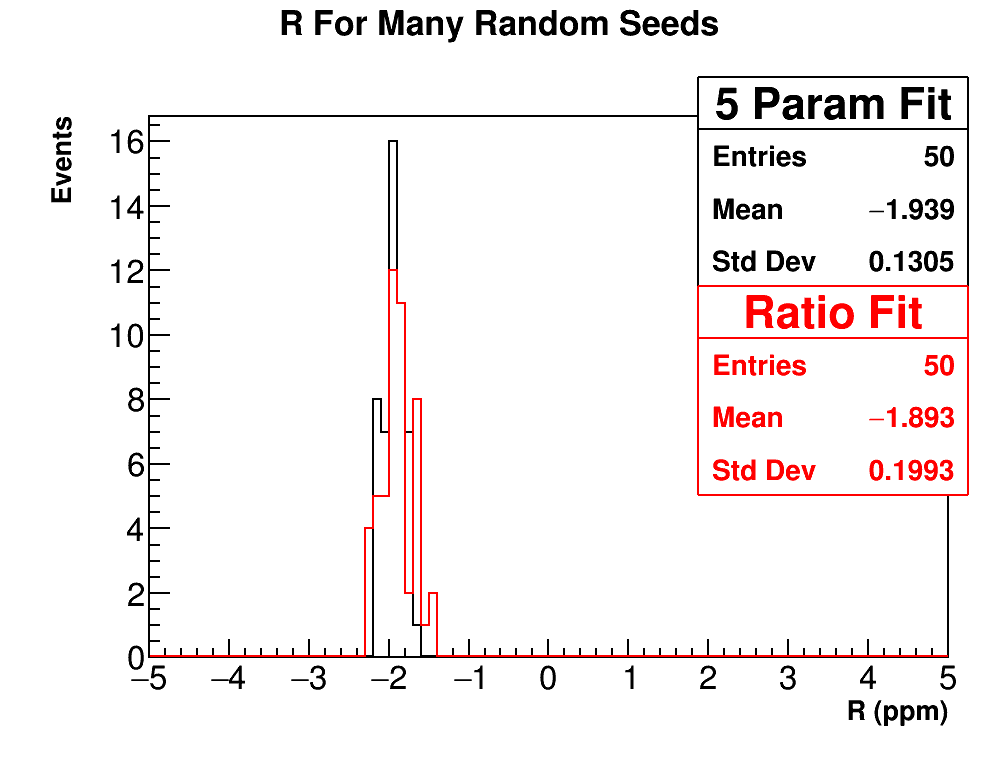
\includegraphics[width=\textwidth]{singleDist_canvas}
	    \caption{Fitted $R$ distribution for a single pseudo-experiment for 5 parameter and 3 parameter ratio fits, for 50 different random seeds.}
	\label{Subfig:SingleRDist}
    \end{subfigure}
   	\hspace{4mm}
    \begin{subfigure}[t]{0.45\textwidth}
	    \centering
		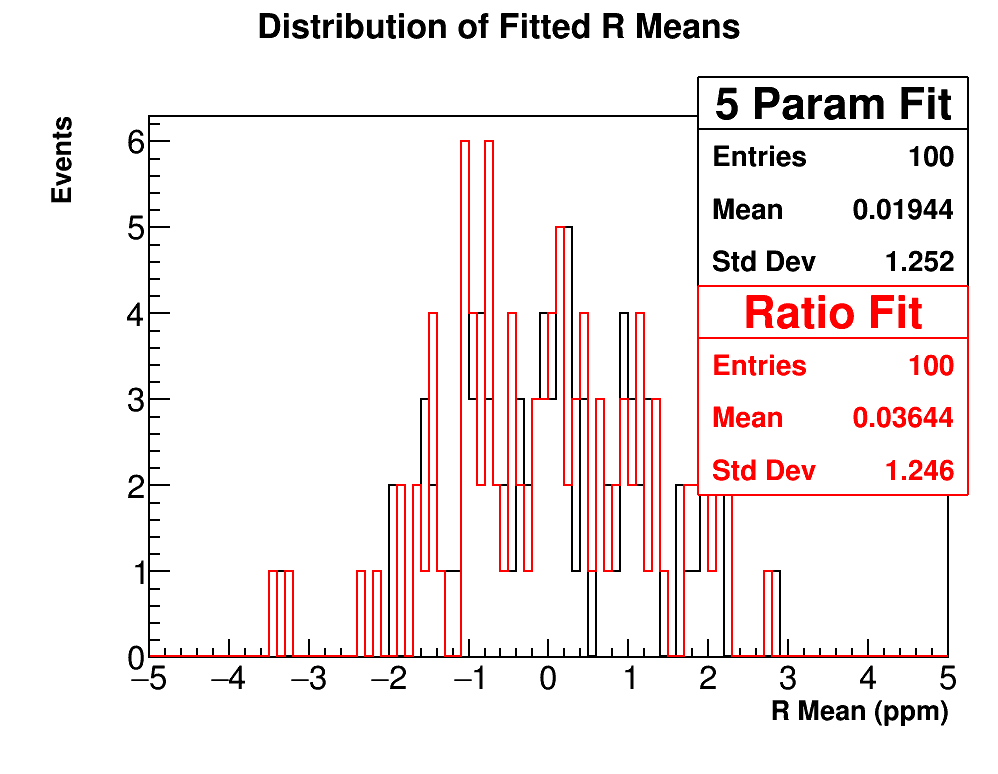
\includegraphics[width=\textwidth]{mean_canvas}
	    \caption{The distribution of means of the fitted $R$ distributions, for 100 separate pseudo-experiments.}
	\label{Subfig:MeanDist}
    \end{subfigure}% %you need this % here to add spacing between subfigures
    \vspace{4mm}
    \begin{subfigure}[t]{0.45\textwidth}
	    \centering
		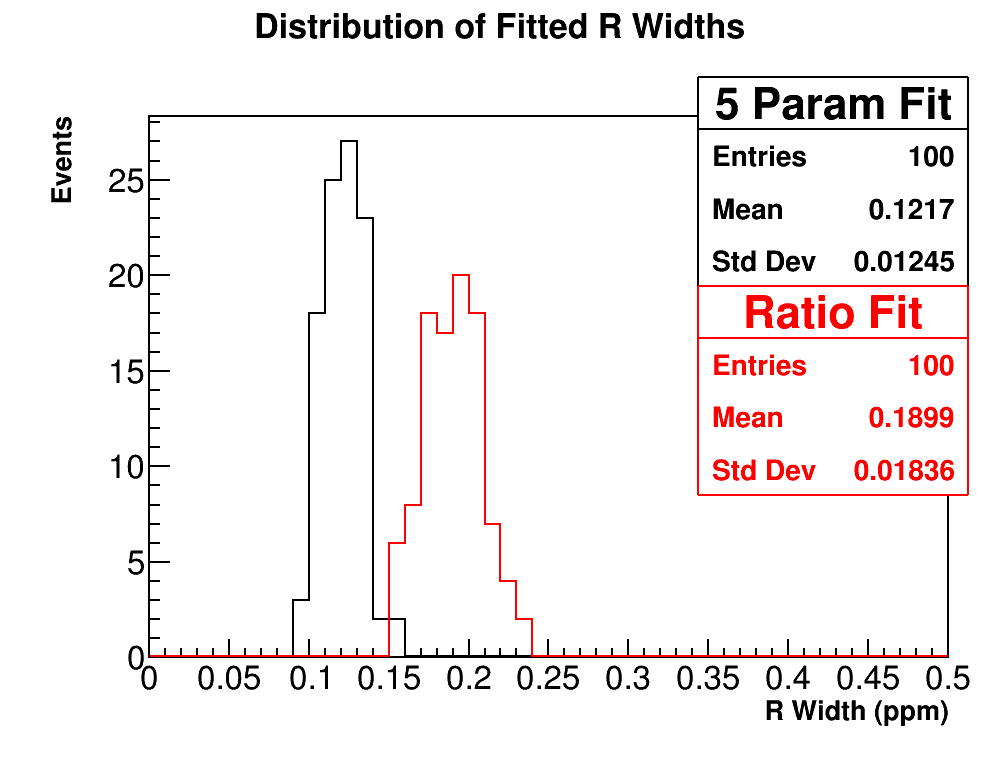
\includegraphics[width=\textwidth]{width_canvas}
	    \caption{The distribution of widths of the fitted $R$ distributions, for 100 separate pseudo-experiments.}
	\label{Subfig:WidthDist}
    \end{subfigure}
   	\hspace{4mm}
    \begin{subfigure}[t]{0.45\textwidth}
	    \centering
		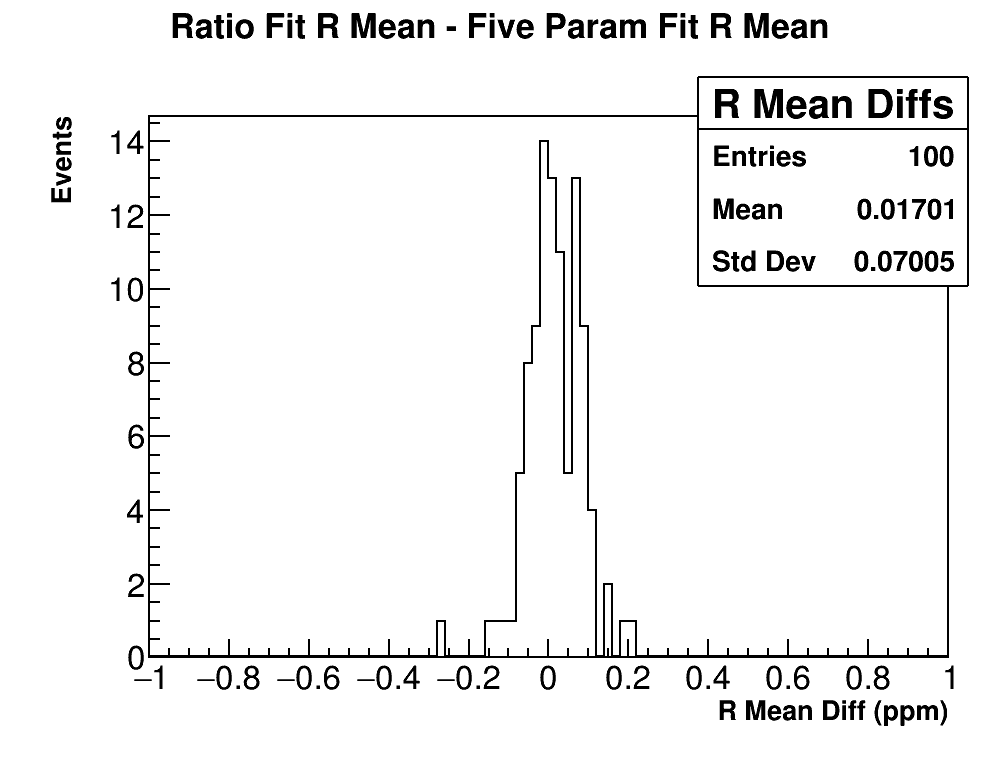
\includegraphics[width=\textwidth]{diff_canvas}
	    \caption{The distribution of differences in fitted $R$ means between 5 parameter fits and 3 parameter ratio fits per pseudo-experiment for 100 pseudo-experiments.}
	\label{Subfig:DiffDist}
    \end{subfigure}% %you need this % here to add spacing between subfigures
\caption[Ratio Method fitted $R$ values compared with T-Method $R$ values in Toy MC with different randomizations]{Toy MC study investigating differences in expected $R$ values between Ratio Method and T-Method fits due to different randomizations. The statistical precision on $R$ for a single fit is approximately \SI{1.3}{ppm}.}
\label{fig:TMethodComparison}
\end{figure}

